% To build, run `tectonic slide.tex`.
% Requires: IPAexMincho font.

% Use beamer.
    \ifdefined\ishandout
        \documentclass[
            unicode,% Use Japanese characters.
            handout,% Generate handout.
        ]{beamer}
    \else
        \documentclass[
            unicode,% Use Japanese characters.
        ]{beamer}
    \fi

% Path variables.
    \newcommand*\commonresourcedir{../../resources}

% Use japanese font.
    \usepackage{zxjatype}
    \usepackage[ipaex]{zxjafont}
% Listing.
    \usepackage{listings}
% Hyper link.
    \usepackage{url}
% Font spec.
    \usepackage{fontspec}
% Use graphics.
    \usepackage{graphicx}

% Beamer theme.
    \usetheme{Antibes}

% Listing preset.
    \lstset{
        language={C++},
        basicstyle={\linespread{0.85}\footnotesize\ttfamily},
        commentstyle={\ttfamily},
    }

% Show "C++" as usual text, prevent + to be treated as addition operator.
    \newcommand*\cpp{C\texttt{++}}

% A slide without headline.
% See https://tex.stackexchange.com/a/45005 .
    \makeatletter
    \newenvironment{withoutheadline}{
        \setbeamertemplate{headline}[default]
        \def\beamer@entrycode{\vspace*{-\headheight}}
    }{}
    \newenvironment{noheadline}{
        \setbeamertemplate{headline}{}
        \addtobeamertemplate{frametitle}{\vspace*{-\headlineheight}}{}
    }{}
    \makeatother

% Insert section page automatically.
    \AtBeginSection[]{
        \begin{noheadline}
            \begin{frame}
                \vfill
                \begin{beamercolorbox}[sep=8pt,center,rounded=true]{title}
                    \usebeamerfont{title}\insertsectionhead\par%
                \end{beamercolorbox}
                \vfill
            \end{frame}
        \end{noheadline}
        \begin{frame}
            \tableofcontents[currentsection]
        \end{frame}
    }
    \AtBeginSubsection[]{
        \begin{noheadline}
            \begin{frame}
                \vfill
                \begin{beamercolorbox}[sep=8pt,center,rounded=true]{title}
                    \usebeamerfont{title}\insertsubsectionhead\par%
                \end{beamercolorbox}
                \vfill
            \end{frame}
        \end{noheadline}
    }

% Custom.
    \newcommand*\hashtag[1]{{\texttt{\#}{#1}}}

\logo{
\includegraphics[width=2cm]{\commonresourcedir/sasori-bg.png}}

\title[文明人]{芝を生やさずに文明を進める方法もあります}
\author{@lo48576 (らりお)}
\institute{ロボット技術研究会}
\date{2017-09-03}

\begin{document}
\frame{\titlepage}

\begin{frame}{今回のもくじ}
    \tableofcontents
\end{frame}

\section{文明}

\subsection{巨人の肩}

\begin{frame}{「巨人の肩に乗る」}
    \begin{quote}
        私たちは巨人の肩の上に乗る小人のようなものだとシャルトルのベルナールは言った。
        私たちが彼らよりもよく、また遠くまでを見ることができるのは、私たち自身の視力が優れているからでもなく、
        ほかの優れた身体的特徴によるのでもなく、ただ彼らの巨大さによって私たちが高く引き上げられているからなのだと。

        \vspace*{\baselineskip}
        \hspace*\fill{\small --- \href{https://ja.wiktionary.org/wiki/\%E5\%B7\%A8\%E4\%BA\%BA\%E3\%81\%AE\%E8\%82\%A9\%E3\%81\%AB\%E7\%AB\%8B\%E3\%81\%A4}{巨人の肩に立つ - ウィクショナリー日本語版}}
    \end{quote}
\end{frame}

\begin{frame}{巨人の肩に乗ろうな!}
    文明に感謝、先人に感謝

    \begin{itemize}
        \item 研究
        \item ソフトウェア開発 ← 今日のお題
        \item その他無数のこと
    \end{itemize}

    以下、明示がなければソフトウェアの文脈で話をします
\end{frame}

\begin{frame}{巨人}
    我々は莫大な既存の資産の上で進捗している

    \begin{itemize}
        \pause
        \item 環境
            \begin{itemize}
                \item OS (Linux, BSD, \ldots)
                \item デスクトップ環境, WM (gnome, KDE, XMonad, i3, \ldots)
                \item シェル (bash, zsh, fish, \ldots)
            \end{itemize}
        \pause
        \item ツール
            \begin{itemize}
                \item エディタ (vim, emacs, \ldots)
                \item コンパイラ (gcc, clang, rustc, ghc, \ldots)
                \item インタプリタ (ruby, python, perl, \ldots)
            \end{itemize}
        \pause
        \item ライブラリ、アプリケーション
            \begin{itemize}
                \item 無数にあるので省略
            \end{itemize}
    \end{itemize}

    OSSに圧倒的感謝!!!
\end{frame}

\begin{frame}{巨人 is 誰}
    我々は誰の肩に立っているのか? \\
    →誰の成果の上で進捗しているのか?

    \begin{itemize}
        \pause
        \item ソフトウェアの開発者
        \pause
        \item ドキュメント著者
        \pause
        \item フォーラムとかでサポートしてる人
        \pause
        \item 解説の本や記事の著者
        \pause
        \item 紹介・布教してた人
    \end{itemize}

    \pause
    \hashtag{人} ~ \hashtag{いろいろな人}
\end{frame}

\subsection{OSSは文明}

\begin{frame}{OSS (FLOSS) is 何}
    Linux, gcc, vim, \ldots などなど、ありがた〜いソフトやライブラリ \\
    これらはすべて \alert{OSS} (FLOSS)

    \begin{itemize}
        \item OSS: オープンソースソフトウェア
        \item FLOSS: Free/Libre and Open Source Software
    \end{itemize}

    {\small (以下、単にOSSというときFLOSSを指すものとする)}
    \vspace*{\baselineskip}

    単にソースコードが公開されているだけで OSS になるわけではない
\end{frame}

\begin{frame}{OSSの思想 (0)}
    正確に説明すると明らかに時間が足りないので大雑把に……\\

    問題点:

    \begin{itemize}
        \pause
        \item ソフトウェア(や、それによって表現されるアルゴリズム等)は、誰でもその恩恵に与れる人類共有の遺産
        \pause
        \item 作者が無闇に権利で縛るのは人類にとっての損失である
            \begin{itemize}
                \pause
                \item 特許で縛ると、本来誰でも使えるはずのソフトウェア技術が使えなくなってしまう
                    \begin{itemize}
                        \item →\href{https://ja.wikipedia.org/wiki/Graphics_Interchange_Format\#.E7.89.B9.E8.A8.B1.E5.95.8F.E9.A1.8C.E3.81.A8.E3.81.9D.E3.81.AE.E9.A1.9B.E6.9C.AB}{GIF形式の特許の騒動}
                    \end{itemize}
                \pause
                \item 著作権で縛ると、作者の都合で人類からソフトウェアを取り上げることができてしまう
                    \begin{itemize}
                        \item →Windowsでありがちな、フリーソフトの公開停止で失われてしまう事案(勝手に再配布すると著作権侵害)
                    \end{itemize}
            \end{itemize}
    \end{itemize}
\end{frame}

\begin{frame}{OSSの思想 (1)}
    OSS(や、そのライセンス)が提示する解決策:

    \begin{itemize}
        \item 作者の権利だけでなく、ユーザ(すなわち潜在的に全人類)の権利と利益を大事にする
            \begin{itemize}
                \pause
                \item たとえば\href{https://www.gnu.org/philosophy/free-sw.ja.html}{自由ソフトウェア}を定義する4つの自由
                    \begin{itemize}
                        \item \alert{どんな目的に対しても、プログラムを望むままに実行する}自由 (第零の自由)。
                        \item プログラムがどのように動作しているか\alert{研究し、必要に応じて改造する}自由 (第一の自由)。
                        \item 身近な人を助けられるよう、\alert{コピーを再配布する}自由 (第二の自由)。
                        \item \alert{改変した版を他に配布する}自由 (第三の自由)。
                    \end{itemize}
                \pause
                \item たとえば\href{https://ja.wikipedia.org/wiki/MIT_License}{MITライセンス} (大雑把に:)
                    \begin{itemize}
                        \item ソフトウェアは、誰でも\alert{無償で無制限}に扱える
                        \item ただし、\alert{著作権表示とライセンス文はちゃんと記載}しろ
                        \item 作者や著作権者は責任を負わない
                    \end{itemize}
            \end{itemize}
    \end{itemize}
\end{frame}

\begin{frame}{OSSのありがたさ}
    \begin{itemize}
        \pause
        \item OSSの上に築いたものは、(他人によって)奪われない
            \begin{itemize}
                \pause
                \item 作者「公開やめるわ」 → 別の有志「我々のプロジェクトで使ってるから同梱して再配布するわ」
                \pause
                \item 作者「OSSにするのやめるわ」 → 別の有志「じゃあ作者でなく我々が改造(アップデート)して別物として公開するわ」
                    \begin{itemize}
                        \item たとえば、OpenALがライセンス変更でOSSでなくなった結果、有志が\href{https://github.com/kcat/openal-soft}{OpenAL Soft}というforkを公開している
                    \end{itemize}
            \end{itemize}
        \pause
        \item OSSは依存やベンダーロックインを強制しない
            \pause
            \begin{itemize}
                \item 「hogeが気に要らんが、作者が直すつもりがないと言っている」→「自分で改造版を公開しよう」
                \item 「fuga言語でしか使えないんだが」→「piyo言語で使えるように移植(改造)しよう」
            \end{itemize}
    \end{itemize}
\end{frame}

\begin{frame}{OSSの闘争}
    ユーザ(人類)の自由を求めて人々が活動している

    \begin{itemize}
        \item GIFに対抗してPNGを開発
        \item MP3に対抗して Ogg Vorbis
        \item MS Office に対抗して OpenOffice.org や LibreOffice
        \item などなど
    \end{itemize}

    OSSに圧倒的感謝!!!
\end{frame}

\section{貢献}

\subsection{貢献してどうなるのか}

\begin{frame}{「コントリビュータ」}
    contribute: 貢献

    定義は曖昧(プロジェクトや組織毎に決まっている場合もある)

    \begin{itemize}
        \item 開発者当人はもちろん
        \pause
        \item コード等がOSSに取り込まれたことのある人とか
        \pause
        \item バグ報告したことがあったり、issue (ticket)を立てたことがある人とか
        \pause
        \item ドキュメントの編集等に携わった人とか
        \pause
        \item 議論に参加した人とか
    \end{itemize}

    \pause
    \alert{貢献とはコードを書くことだけではない}
\end{frame}

\begin{frame}{OSSに貢献する人々}
    思い出そう、 ~ \hashtag{いろいろな人}

    \begin{itemize}
        \item ソフトウェアの開発者
        \item ドキュメント著者
        \item フォーラムとかでサポートしてる人
        \item 解説の本や記事の著者
        \item 紹介・布教してる人
    \end{itemize}
\end{frame}

\begin{frame}{貢献の意義}
    なぜ ~ \hashtag{いろいろな人} ~ が発生するのか

    \begin{itemize}
        \pause
        \item 建前/崇高なやつ/思想
            \begin{itemize}
                \item 人々が参考にできる情報や技術を蓄積・進歩させる
                \item 人々が使える道具を増やし、またより便利にする
                \item OSSの利用者や開発者を助ける
                \item 世話になったOSSへの\alert{恩返し}
            \end{itemize}
        \pause
        \item 本音/利益になるやつ
            \begin{itemize}
                \item 技術力の誇示
                \item 自身のブランド化・コンテンツ化 ←これはっょぃ人用
                \item OSSを(一部分であれ)自分好みにできる場合がある
                \item \alert{自分の使ってる道具を便利にする}
                \item 自己満足
            \end{itemize}
    \end{itemize}
\end{frame}

\begin{frame}{貢献の方法}
    \begin{tabular}{l|l} \hline
        \hashtag{人}            & 方法 \\ \hline
        ソフトウェアの開発者    & ソフトウェアを開発する \\ \hline
        ドキュメント編集者      & \shortstack{ドキュメントを書く、\\修正する、\alert{翻訳する}} \\ \hline
        \shortstack{フォーラムとかで\\サポートしてる人}    & フォーラムで議論やサポートをする \\ \hline
        解説の本や記事の著者    & 解説記事等を書く \\ \hline
        紹介・布教してる人      & 紹介・布教する \\ \hline
    \end{tabular}
\end{frame}

\subsection{私の場合}

\begin{frame}{紹介・布教する}
    \begin{itemize}
        \pause
        \item 「××はいいぞ」と \href{http://twilog.org/lo48576/search?word=Rust\%20\%E3\%81\%AF\%E3\%81\%84\%E3\%81\%84\%E3\%81\%9E&ao=a}{twitter で連呼するとか}
            \begin{itemize}
                \item 知名度は大事
            \end{itemize}
        \pause
        \item 積極的な声かけ: 「ところで gentoo linux という素晴らしいディストリビューションがあるのですが……」
            \begin{itemize}
                \item 身近な範囲で手厚いサポートを
            \end{itemize}
        \pause
        \item ブログとか書くとか
            \begin{itemize}
                \item \href{http://titech-ssr.blog.jp/archives/1013311908.html}{普通の東工大生が【gentoo】入れてみた。 : 東京工業大学 ロボット技術研究会}
            \end{itemize}
    \end{itemize}
\end{frame}

\begin{frame}{解説等を書く}
    布教に通じるものがある

    \begin{itemize}
        \pause
        \item 手っ取り早いのはブログ
            \begin{itemize}
                \item \href{https://blog.cardina1.red/2017/04/13/federated-social-web/}{gnusocial や mastodon の哲学 - 何とは言わない天然水飲みたさ}
                \item \href{https://blog.cardina1.red/2016/12/06/kernel-config-shellscript/}{kernel config 生成(略記)のためのシェルスクリプト - 何とは言わない天然水飲みたさ}
            \end{itemize}
        \pause
        \item Qiitaのような専用サイトもある
            \begin{itemize}
                \item \href{http://qiita.com/lo48576/items/34887794c146042aebf1}{Rustのイテレータの網羅的かつ大雑把な紹介 - Qiita}
                \item \href{http://qiita.com/lo48576/items/343ca40a03c3b86b67cb}{Rustでf32やf64の配列の最大値を得る方法 - Qiita}
            \end{itemize}
        \pause
        \item 内容は様々
            \begin{itemize}
                \item 理念や概念の解説
                \item トラブルシューティング
                \item 布教
            \end{itemize}
        \pause
        \item 同人誌等を出すのも良い
    \end{itemize}
\end{frame}

\begin{frame}{フォーラムとかでサポートしてる人}
    \begin{itemize}
        \item すごいですね。
        \pause
        \item 私はフォーラムで何か書いた経験がほとんど無いので、経験から語れることは特にない
        \item べつにフォーラムじゃなくてtwitterとかで疑問に答えるくらいから始めたって良い
    \end{itemize}
\end{frame}

\begin{frame}{ドキュメント編集}
    \begin{itemize}
        \item 翻訳
            \begin{itemize}
                \item wiki や修正だと、用語等を合わせるのに多少気をつかう
                \item ドキュメントが大規模でなかったり、一番乗りの翻訳だったりすると、やりやすい(かも)
            \end{itemize}
    \end{itemize}
    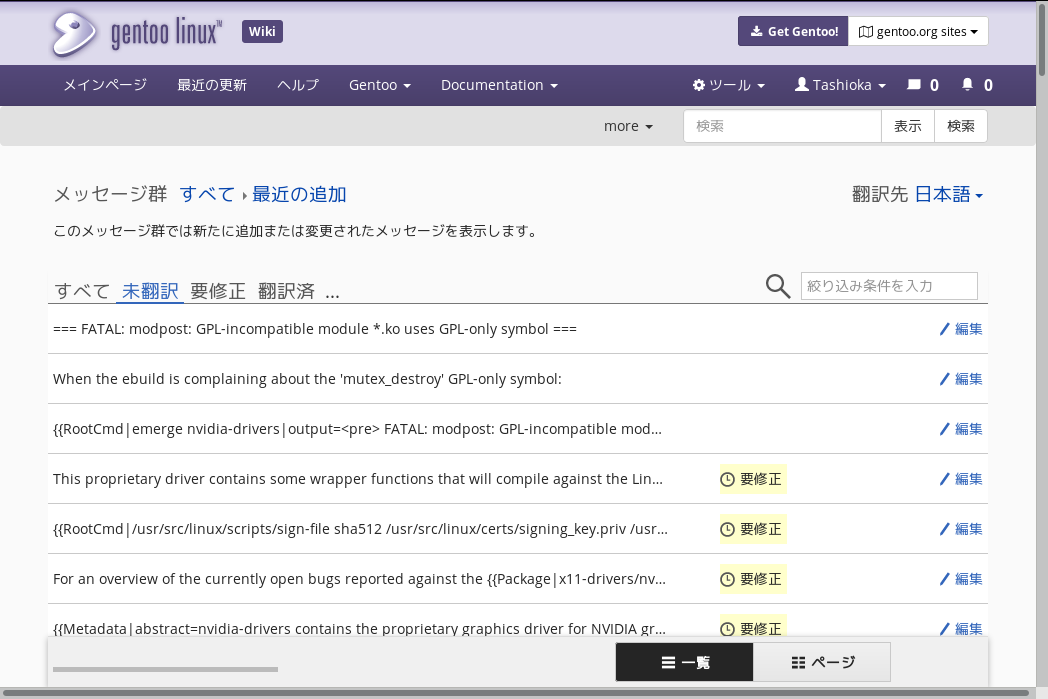
\includegraphics[width=0.5\textwidth]{images/gentoo-wiki-translation-tool.png}
    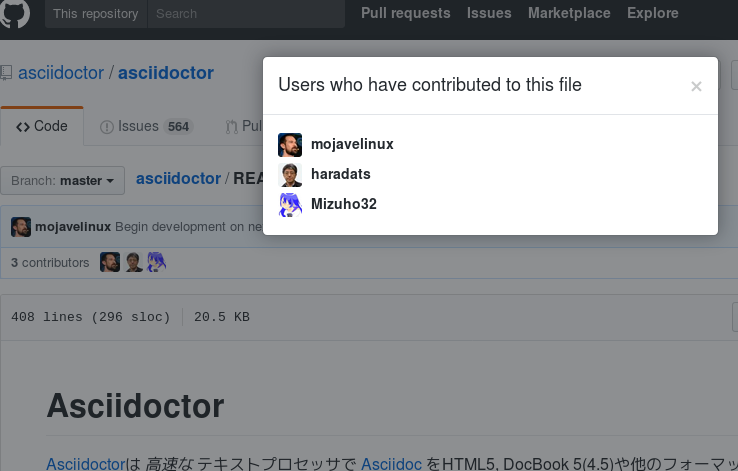
\includegraphics[width=0.5\textwidth]{images/asciidoctor-mizuho32.png}
\end{frame}

\begin{frame}{ドキュメント編集}
    \begin{itemize}
        \item 修正
            \begin{itemize}
                \item
                    \href{https://github.com/rust-lang-nursery/rust-clippy/issues/1232}{ドキュメントの些細なミス}を\href{https://github.com/rust-lang-nursery/rust-clippy/pull/1233}{修正}したり
                \item \href{https://github.com/ivanceras/rustorm/issues/31}{疑問があったら質問する}だけでも良い
                    \begin{itemize}
                        \item 後で同じ疑問を持った人が、質問せず検索するだけで答えに辿りつけるようになるので、十分に有意義
                    \end{itemize}
            \end{itemize}
        \pause
        \item 修正にせよ新規にせよ、英語で書くつもりなら、それなりのエーゴ力は欲しい……
    \end{itemize}
\end{frame}

\begin{frame}{ソフトウェア開発: 質問を投げる、機能を要望する (0)}
    曖昧な場合: 「こんな機能ない?」「これしたいんだけど、どうすればいい?」

    \begin{itemize}
        \item \href{https://github.com/jaor/xmobar/issues/301}{Feature request: relative width, absolute height · Issue \#301 · jaor/xmobar}
            \begin{itemize}
                \item 「うん、いいね」「まてよ、既にあるじゃん」と言われた(完)
            \end{itemize}
    \end{itemize}
\end{frame}

\begin{frame}{ソフトウェア開発: 質問を投げる、機能を要望する (1)}
    明確な場合: 「こういう挙動の機能が欲しい!」

    \begin{itemize}
        \item \href{https://github.com/nabijaczleweli/cargo-update/issues/25}{Toolchain and options settings for each crate · Issue \#25 · nabijaczleweli/cargo-update}
            \begin{itemize}
                \pause
                \item 開発者「軽く検討してみたけど、hogeがつらいし複雑度も激増しそう……それともなんかいいアイデアでもある?」
                \pause
                \item 私「既存ツールにこんな感じでhogeしてるやつらあるし、言うほど複雑にはならなそうじゃない?」
                \pause
                \item 開発者「できそうだしやってみるわ」
                \pause
                \item 開発者「できたけどどう?」
                \pause
                \item 私「ヘルプがおかしいで」「アップデート時だけでなく初回インストール時にもfugaしてほしいな」
                \pause
                \item 開発者「実装と修正したよ」
                \pause
                \item 私「short option ちょうだい」
                \pause
                \item 開発者「はい」
                \item 私「ありがとう!」

            \end{itemize}
    \end{itemize}
\end{frame}

\begin{frame}{ソフトウェア開発: 質問を投げる、機能を要望する (2)}
    明確な場合: 「こういう機能欲しい!」(←我慢できない顔)

    \begin{itemize}
        \item
            \href{https://github.com/Peternator7/strum/issues/9}{Implement \`{}AsRef<str>\`{}? · Issue \#9 · Peternator7/strum}, \\
            \href{https://github.com/Peternator7/strum/pull/10}{Add \`{}derive(AsRefStr)\`{} implementation by lo48576 · Pull Request \#10 · Peternator7/strum}
            \begin{itemize}
                \item 私「ほしい!」
                \pause
                \item 私「我慢できへんかったんで実装した」「ドキュメントは書いてないけどごめんね」「hogeが自信ないんだけどどう思う?」
                \pause
                \item 開発者「いいじゃん」「poyoいらなくない?」「hogeはfugaの方がいいかな」
                \pause
                \item 私「あいよ直した」
                \pause
                \item 開発者「取り込んだのでドキュメント書いたらバージョン上げるぜ」
            \end{itemize}
    \end{itemize}
\end{frame}

\begin{frame}{ソフトウェア開発: 報告する (0)}
    害ではないが不審な挙動・設計: 「この挙動が妙なんだけど、こうした方が良いのでは?」

    \begin{itemize}
        \pause
        \item \href{https://github.com/nagisa/rust_libloading/issues/22}{Unwanted \`{}println!\`{} debug print? · Issue \#22 · nagisa/rust\_libloading}
            \begin{itemize}
                \item 私「おかしくない?」
                \item 開発者「せやな、直した」
            \end{itemize}
        \pause
        \item \href{https://github.com/slog-rs/slog/issues/119}{\`{}Logger::to\_erased()\`{} should not consume \`{}self\`{} · Issue \#119 · slog-rs/slog}
            \begin{itemize}
                \item 私「この関数って本来こう在るべきだよね」
                \item 開発者「せやな」→直った
            \end{itemize}
    \end{itemize}
\end{frame}

\begin{frame}{ソフトウェア開発: 報告する (1)}
    明らかに駄目なタイプの挙動・設計: 「これ駄目なやつなんだけど」

    \begin{itemize}
        \item \href{https://github.com/neovim/neovim/issues/6178}{shell script is not highlighted correctly when a default value of a variable is specified · Issue \#6178 · neovim/neovim}
            \begin{itemize}
                \item 私「neovimのシンタックスハイライトがおかしいが(vimでは正常やで)」
                \pause
                \item 開発者「これvimのを流用してる部分だから、vimで直ってるならneovimでもそのうち直るで」(完)
            \end{itemize}
    \end{itemize}
\end{frame}

\begin{frame}{ソフトウェア開発: 修正する}
    バグの修正とか。

    \begin{itemize}
        \item
            \href{https://github.com/dylanede/rusttype/pull/14}{大}%
            \href{https://github.com/dylanede/rusttype/pull/15}{抵}%
            \href{https://git.gnu.io/gnu/gnu-social/merge_requests/145}{の}%
            \href{https://git.gnu.io/h2p/Qvitter/merge_requests/101}{例}

            \begin{itemize}
                \item 私「直したで」
                \item 開発者「Thank you」(または無言)
            \end{itemize}
        \item
            \href{https://github.com/reem/rust-ordered-float/pull/28}{よく}%
            \href{https://gitgud.io/panjoozek413/qvitterplus/merge_requests/3}{ある}%
            例
            \begin{itemize}
                \item 私「直したで」
                \item 開発者「……」(一切の反応なし)
            \end{itemize}
            \pause
            →そもそも開発者の芝が生えてないことも多い(かなしい)
    \end{itemize}
\end{frame}

\begin{frame}{ソフトウェア開発: 改善する}
    どう考えても良くできる部分: 「こうならない理由がないよね」

    \begin{itemize}
        \item \href{https://github.com/dylanede/rusttype/pull/22}{Use better (longer) lifetime as possible for \`{}Font\`{} by lo48576 · Pull Request \#22 · dylanede/rusttype}
            \begin{itemize}
                \item 私「参照の寿命の制約、もっと緩くできるよね」
                \item 開発者「せやな」
            \end{itemize}
        \item \href{https://github.com/alexcrichton/flate2-rs/pull/52}{Remove unnecessary trait bounds from reader types definitions by lo48576 · Pull Request \#52 · alexcrichton/flate2-rs}
            \begin{itemize}
                \item 私「型パラメータの制約弱くできるよね」
                \item 開発者「Thanks」
            \end{itemize}
        \item \href{https://github.com/dylanede/rusttype/pull/16}{Update dependencies by lo48576 · Pull Request \#16 · dylanede/rusttype}
            \begin{itemize}
                \item 私「依存が古すぎてアレだから新しいの使ってくれ」
            \end{itemize}
            →他の Pull Request で使う都合もあった
    \end{itemize}
\end{frame}

\begin{frame}{ソフトウェア開発: 自分のプロジェクトを作る}
    ないものは作る \\
    (あっても作っていい)

    \begin{itemize}
        \item 私の場合、FBX関連とか……
        \item 自分で使う用なので、他人からの評価は割とどうでもいい
        \item が、Starが付くと地味に嬉しい
    \end{itemize}
\end{frame}

\begin{frame}{何故プロジェクトを公開するか?: 開発者}
    個人規模で管理されているプロジェクトが公開されていると、開発者は何が嬉しいのか

    \begin{itemize}
        \pause
        \item 他人の知恵(contribute)を貰える場合がある
        \pause
        \item 使いやすくなる
            \begin{itemize}
                \item 整理して公開されていると、時間が経っても使いやすい
                \item ライブラリ等は、アプリケーションと疎結合にして公開することになるので、他へ応用しやすい
            \end{itemize}
        \pause
        \item 大規模になっても、ユーザが増えると開発に参加してくれる人が増えるかも
            \begin{itemize}
                \item Mastodon とかそんな感じ
            \end{itemize}
        \pause
        \item 開発を止めても、他の誰かが引き継いでくれるかも
            \begin{itemize}
                \item 本家のリポジトリを明け渡すこともある
                \item 本家はそのままでforkの開発が活発になる場合もある
            \end{itemize}
    \end{itemize}
\end{frame}

\begin{frame}{何故プロジェクトを公開するか?: 開発者以外}
    個人規模で管理されているプロジェクトが公開されていると、開発者は何が嬉しいのか

    \begin{itemize}
        \pause
        \item 自分で作らずとも他人の成果物が使えるかもしれない
        \item 自分で何か作るときの参考になるかもしれない
        \pause
        \item 勉強に使える
        \pause
        \item 使ってみての不満等を改善しやすい
        \item 問題があったとき修正の状況を追える
    \end{itemize}
\end{frame}

\subsection{これからOSSへ貢献してみたい人は}

\begin{frame}{何に?}
    \begin{itemize}
        \pause
        \item 自分が使うOSS
            \begin{itemize}
                \item 間接的な依存先も含む
            \end{itemize}
        \pause
        \item 支援・応援したいOSS
        \pause
        \item 問題を見付けてしまったもの
            \begin{itemize}
                \item 修正できるなら修正すればおk
                \item 問題なかった場合「それ仕様」とか言ってもらえるから大丈夫
            \end{itemize}
    \end{itemize}

    \pause
    ただし:

    \begin{itemize}
        \item 大規模プロジェクトはそれなりに難しいので注意が必要
            \begin{itemize}
                \item 注意というか、知識が必要
                \item 貢献の様式があったりする
            \end{itemize}
    \end{itemize}
\end{frame}

\begin{frame}{どうやって?}
    \begin{itemize}
        \item 先述のとおり、いろいろな方法で
        \pause
        \item ルールを守る
            \begin{itemize}
                \pause
                \item issueは既に重複がないか、先に確認する
                    \begin{itemize}
                        \item 調べるのが難しければ、フォーラムとかで聞くのもありかも
                        \item もし重複でissueを立ててしまっても、大抵は気付かれる(ただし余計な手間をかけてしまう)
                    \end{itemize}
                \pause
                \item Code of conduct (行動規範)やCONTRIBUTINGファイルやREADMEに、ルールや貢献方法が書いてある場合がある
                    \begin{itemize}
                        \item たとえば: 機能提案はissueではなくRFCsリポジトリにファイルを置いて提出し議論せよ、など
                    \end{itemize}
                \pause
                \item パッチや翻訳を投げるなら、著作権やライセンス関連の扱いに注意
                    \begin{itemize}
                        \item コピペは大抵アウト
                        \item 自動翻訳を投げるのもアウトなことがとても多い
                    \end{itemize}
            \end{itemize}
    \end{itemize}
\end{frame}

\begin{frame}{でも……}
    \begin{itemize}
        \pause
        \item 自分ごときのソフトウェアを公開しても意味がない?
            \begin{itemize}
                \pause
                \item 意味を見出すのはあなただけではない
                \item 数年後に検索でやってきてコード片を読んだ人が何かを学べるかもしれない
                \item 界隈の人気の指標にも使える
            \end{itemize}
        \pause
        \item 公開するほどの品質がない?
            \begin{itemize}
                \pause
                \item 「自分用」「not production ready」など注記を付けて公開しよう
                \item 他人に読めないコードはいずれ自分にも読めなくなるので、日頃から真っ当に書こう (3日後の自分は他人)
                \item 他人のためのドキュメント等を書く技術はいずれ役に立つ
            \end{itemize}
    \end{itemize}
\end{frame}

\begin{frame}{}
    \phantom{}
    {\Large\centering
        あなたとOSS,\\
        今すぐコントリビュー\\
        ト\\
    }
\end{frame}

\section*{おまけ}

\begin{frame}{参考文献}
    \begin{itemize}
        \item OSSライセンス
            \begin{itemize}
                \item \href{https://www.gnu.org/philosophy/free-sw.ja.html}{自由ソフトウェアとは? - GNUプロジェクト - フリーソフトウェアファウンデーション}
                \item \href{http://postd.cc/mit-license-line-by-line/}{MITライセンスを1行1行読んでいく | プログラミング | POSTD}
            \end{itemize}
        \item OSSへ貢献してみようという話
            \begin{itemize}
                \item \href{https://melborne.github.io/2014/01/23/contribute-to-english-based-opensource-project-or-sinatra-japanese-readme/}{英語圏のオープンソースプロジェクトに貢献する最も簡単な方法またはsinatra/README.jp.mdまたは彼はなぜ私を愛するようになったか}
                \item \href{https://medium.com/@timakin/\%E4\%BB\%8A\%E5\%B9\%B4\%E3\%81\%AF-\%E4\%BD\%95\%E3\%81\%8B\%E5\%A4\%A7\%E3\%81\%8D\%E3\%82\%81\%E3\%81\%AEoss\%E3\%81\%AB\%E3\%82\%B3\%E3\%83\%B3\%E3\%83\%88\%E3\%83\%AA\%E3\%83\%93\%E3\%83\%A5\%E3\%83\%BC\%E3\%83\%88\%E3\%81\%97\%E3\%81\%9F\%E3\%81\%84\%E3\%81\%A7\%E3\%81\%99\%E3\%81\%AD-902771f0ba0e}{「今年は…何か大きめのOSSにコントリビュートしたいですね」 – timakin – Medium}
                \item \href{http://www.atmarkit.co.jp/ait/articles/1211/28/news006.html}{オープンソースコミッタへの道:「使う」から「公開する」へ (1/2) - @IT}
            \end{itemize}
    \end{itemize}
\end{frame}

\begin{frame}{LICENSE}
    \phantom{}
    {
        \centering
        
\includegraphics[width=0.4\linewidth]{\commonresourcedir/cc-by-4_0.pdf}\\
    }

    \vspace*{\baselineskip}
    このドキュメントは\href{http://creativecommons.org/licenses/by/4.0/}{クリエイティブ・コモンズ 表示 4.0 国際 ライセンス}の下に提供されています。
\end{frame}

\end{document}
